\section{使用示例}
大学与城市共生共荣共成长。广州大学是以国家重要中心城市“广州”命名的综合性大学,于2000年合并组建,有着90多年的办学传统。

参考文献\upcite{冯云乔2018}。

\subsection{二级标题1}
大学与城市共生共荣共成长。广州大学是以国家重要中心城市“广州”命名的综合性大学,于2000年合并组建,有着90多年的办学传统。

\subsection{二级标题2}
大学与城市共生共荣共成长。广州大学是以国家重要中心城市“广州”命名的综合性大学,于2000年合并组建,有着90多年的办学传统。

\subsubsection{三级标题1}
大学与城市共生共荣共成长。广州大学是以国家重要中心城市“广州”命名的综合性大学,于2000年合并组建,有着90多年的办学传统。

\subsubsection{三级标题2}
大学与城市共生共荣共成长。广州大学是以国家重要中心城市“广州”命名的综合性大学,于2000年合并组建,有着90多年的办学传统。

\subsubsection{三级标题3}
大学与城市共生共荣共成长。广州大学是以国家重要中心城市“广州”命名的综合性大学,于2000年合并组建,有着90多年的办学传统。

\subsubsection{三级标题4}
大学与城市共生共荣共成长。广州大学是以国家重要中心城市“广州”命名的综合性大学,于2000年合并组建,有着90多年的办学传统。

\paragraph{四级标题1}
大学与城市共生共荣共成长。广州大学是以国家重要中心城市“广州”命名的综合性大学,于2000年合并组建,有着90多年的办学传统。

\paragraph{四级标题2}
大学与城市共生共荣共成长。广州大学是以国家重要中心城市“广州”命名的综合性大学,于2000年合并组建,有着90多年的办学传统。

\subsubsection{三级标题5}
大学与城市共生共荣共成长。广州大学是以国家重要中心城市“广州”命名的综合性大学,于2000年合并组建,有着90多年的办学传统。


\subsection{公式}

行内公式$a^2+b^2=z$,行间公式:
\begin{equation}\label{eq121212}
	x^2+y^2=100
\end{equation}


\subsection{表格}

\begin{table}[htbp]
	\centering
	\caption{Add caption}	\label{tab:1}%
	\begin{tabular}{|c|c|c|c|c|c|c|c|c|c|c|c|c|c|c|}
		\hline
		A           & B           & C           & D           & E           & F           & G           & H           & I           & J           & K           & L           & M           & N           & O \bigstrut\\
		\hline
		1           & 2           & 3           & 4           & 5           & 6           & 7           & 8           & 9           & 10          & 11          & 12          & 13          & 14          & 15 \bigstrut\\
		\hline
		$\alpha$        & $\beta$        & $\gamma$        & $\delta$        & $\epsilon$        & $\varepsilon$        & $\zeta$        & $\eta$        & $\theta$        & $\vartheta$        & $\iota$        & $\kappa$        & $\lambda$        & $\mu$        & $\nu$ \bigstrut\\
		\hline
		$\bowtie$        & $\Join$        & $\propto$        & $\varpropto$        & $\multimap$        & $\pitchfork$        & $\therefore$        & $\because$        & $\neq$        & $\equiv$        & $\approx$        & $\sim$        & $\nsim$        & $\simeq$        & $\backsimeq$ \bigstrut\\
		\hline
	\end{tabular}
\end{table}


\begin{table}[!htbp]
	\centering
	\caption{Add caption}	\label{tab:2}%
	\begin{tabular}{cccccccccc}
		\toprule
		A           & B           & C           & D           & E \\
		\midrule
		1           & 2           & 3           & 4           & 5  & 6           & 7           & 8           & 9           & 10\\
		a           & b           & c           & d           & e &A           & B           & C           & D           & E\\
		A           & B           & C           & D           & E &a           & b           & c           & d           & e \\
		\bottomrule
	\end{tabular}
\end{table}


\subsection{图片}

\begin{figure}[!htb]
	\centering
	
\includegraphics[width=3cm]{广大校徽}
	\caption{广州大学校徽}
	\label{fig:01}
\end{figure}

大学与城市共生共荣共成长。广州大学是以国家重要中心城市“广州”命名的综合性大学,于2000年合并组建,有着90多年的办学传统。
\begin{figure}[!htb]
	\centering
	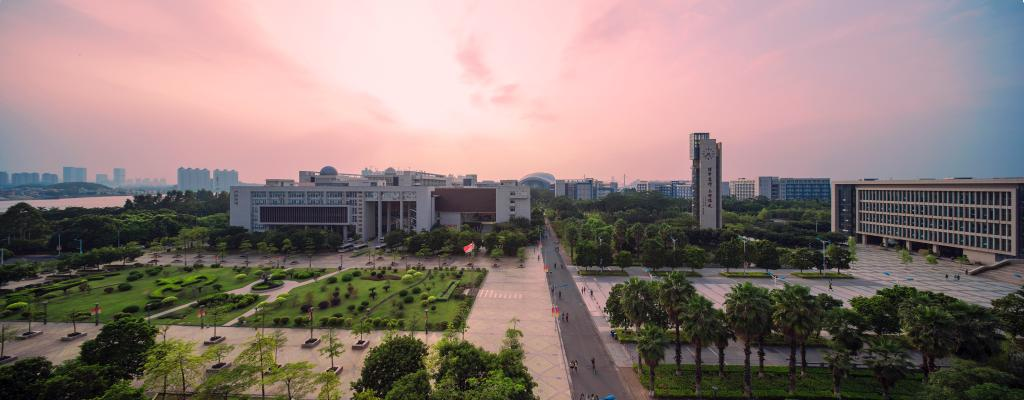
\includegraphics[width=0.7\linewidth]{广场校训塔}
	\caption{广场校训塔}
	\label{fig:2}
\end{figure}







\subsection{参考文献}

若不需要上标,直接使用\verb*|\cite{bibid}|,效果为\cite{Armstrong2006,王先甲2018}。

当需要使用上标时,使用\verb*|\upcite{bibid}|,效果为\upcite{Armstrong2006,王先甲2018}。


同时引用多篇文献\upcite{NBERw25015,陈国青2018, 张彩霞2018,郭韧2018, 丁胜红2019, 申静2019, Xu2019},中间出现不连续文献时\upcite{王先甲2018,马琳2019, 李永立2020,  史丽丽2020, 陈国青2018, 张彩霞2018, 郭韧2018, 丁胜红2019, 申静2019, Xu2019}。




